%!TEX program = xelatex

%%%%%%%%%%%%%%%%%%%%%%%%%%%%%%%%%%%%%%%%%
% Devesh Khandelwal Resume/CV
% XeLaTeX Template
% Version 1.2 (3/5/15)
%
% This template has been downloaded from:
% http://www.LaTeXTemplates.com
%
% Original author:
% Adrien Friggeri (adrien@friggeri.net)
% https://github.com/afriggeri/CV
% 
% Modified by:
% Devesh Khandelwal
% Github: @devkhan
%
% License:
% CC BY-NC-SA 3.0 (http://creativecommons.org/licenses/by-nc-sa/3.0/)
%
% Important notes:
% This template needs to be compiled with XeLaTeX and the bibliography, if used,
% needs to be compiled with biber rather than bibtex.
%
%%%%%%%%%%%%%%%%%%%%%%%%%%%%%%%%%%%%%%%%%

\documentclass[]{devkhan-cv} % Add 'print' as an option into the square bracket to remove colors from this template for printing

\addbibresource{bibliography.bib} % Specify the bibliography file to include publications

\begin{document}

\header{devesh}{khandelwal}{learner} % Your name and current job title/field

%----------------------------------------------------------------------------------------
%	SIDEBAR SECTION
%----------------------------------------------------------------------------------------

\begin{aside} % In the aside, each new line forces a line break
	\section{contact}
		319, CPWD Quarters
		CGRC, Dev Nagar
		Delhi, India
		~
		+91 9810 297 002
		~
		\href{mailto:devesh.khandelwal@outlook.com}{devesh.khandelwal
			@outlook.com}
		\href{http://devkhan.github.io}{devkhan.github.io}
	\section{languages}
		hindi mother tongue
		english
	\section{programming}
		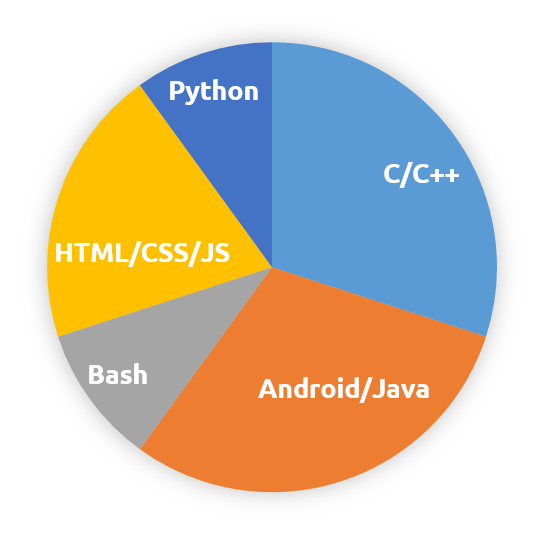
\includegraphics[scale=0.35]{img/programming.png}
		%{\color{red} $\varheartsuit$} C/C++
		%C\# JavaScript
		%HTML5 \& CSS3
	\section{technologies}
		Android, Web UI, WPF, REST API, GNU Tools, SQL, Flask, MVC
\end{aside}

%----------------------------------------------------------------------------------------
%	EDUCATION SECTION
%----------------------------------------------------------------------------------------

\section{education}
	\begin{entrylist}

		\entry
			{2013-Present}
			{Graduation}
			{Cluster Innovation Centre, University of Delhi, Delhi}
			{\small Bachelor of Technology\\Information Technology and Mathematical Innovations}
			

		\entry
			{2010}
			{High School}
			{Central Board of Secondary Education, Delhi}
			{\small AISSE-2010}

		\entry
			{2012}
			{Intermediate}
			{Central Board of Secondary Education, Delhi}
			{\small AISSCE-2012}

	\end{entrylist}

%----------------------------------------------------------------------------------------
%	WORK EXPERIENCE SECTION
%----------------------------------------------------------------------------------------

\section{experience}
	\begin{entrylist}

		\entry
			{2014}
			{General Commerce Limited}
			{Noida, Uttar Pradesh}
			{\emph{Summer Intern (July-August)} \\
				Worked in a group of students from my own college, towards the strategic IT Alignment of the company under the IT Maha Abhiyan initiative of the University of Delhi, PHD Chamber and IamSMEofIndia. Work done: \\
			\begin{itemize}
				\item Learned about the flow of working in a manufacturing company, garment export industry and did business and technological analysis.
				\item Built the company website and also online presence on social networks.
				\item Became familiar with their ERP implementation and also helped other employees.
			\end{itemize}
			}

	\end{entrylist}

%----------------------------------------------------------------------------------------
%	AWARDS SECTION
%----------------------------------------------------------------------------------------

\section{projects}
	\begin{entrylist}

		\entry
			{2015}
			{University of Delhi}
			{Delhi}
			{\emph{Antardhvani Official App} \\
			Developed the official mobile application for the Antardhvani 2015, the official annual festival of Univeristy of Delhi in collaboration with a team of developers.}

	\end{entrylist}

%----------------------------------------------------------------------------------------
%	COURSEWORK SECTION
%----------------------------------------------------------------------------------------

\section{coursework}
	\begin{entrylist}

		\entry
			{\textbf{it \& computing:}}
			{}{}{programming, data structures, algorithms, database management, computation	theory, operating systems}

		\entry
			{\textbf{mathematics:}}
			{}{}{calculus, linear algebra, discrete mathematics, probability \& statistics, mathematical modelling, combinatory logic}

		\entry
			{\textbf{biology:}}
			{}{}{cell biology, molecular biology, integrative biology, genetics \& genomics}

	\end{entrylist}

\end{document}
================================== THE END ==================================%